\documentclass[tikz, border=10pt]{standalone}
\usepackage{tikz}
\usetikzlibrary{decorations.pathmorphing, patterns}

\begin{document}
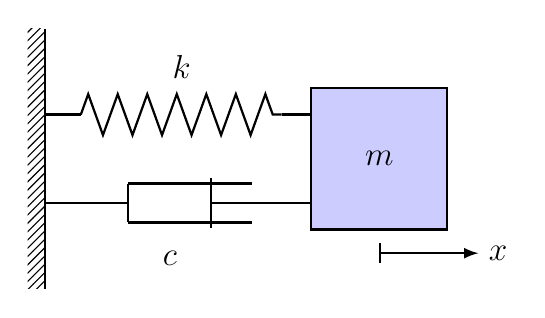
\begin{tikzpicture}[thick, >=latex]

  % --- Wall ---
  \fill[pattern=north east lines] (-0.225, -1.65) rectangle (0, 1.65);
  \draw (0, -1.65) -- (0, 1.65);

  % --- Mass ---
  \fill[blue!20] (3.375, -0.9) rectangle (5.1, 0.9);
  \draw         (3.375, -0.9) rectangle (5.1, 0.9);
  \node[font=\large] at (4.24, 0) {$m$};

  % --- Spring (upper) ---
  \draw (0, 0.56) -- (0.45, 0.56);
  \draw[decorate, decoration={zigzag, segment length=3.75mm, amplitude=2.6mm}]
        (0.45, 0.56) -- (3.0, 0.56);
  \draw (3.0, 0.56) -- (3.375, 0.56);
  \node[font=\large, above=6pt] at (1.73, 0.68) {$k$};

  % --- Damper (lower) ---
  % line from wall to cylinder
  \draw (0, -0.56) -- (1.05, -0.56);
  % cylinder body (open on right)
  \draw (1.05, -0.315) -- (1.05, -0.81);   % left end cap
  \draw (1.05, -0.81)  -- (2.625, -0.81);  % bottom wall
  \draw (1.05, -0.315) -- (2.625, -0.315); % top wall
  % piston plate (extends slightly beyond cylinder walls)
  \draw (2.1, -0.24) -- (2.1, -0.885);
  % rod from piston to mass
  \draw (2.1, -0.56) -- (3.375, -0.56);
  \node[font=\large, below=6pt] at (1.58, -0.83) {$c$};

  % --- x direction arrow ---
  \draw[|->] (4.24, -1.2) -- (5.5, -1.2) node[font=\large, right] {$x$};

\end{tikzpicture}
\end{document}
